\documentclass[12pt,a4paper]{article}
\usepackage[utf8]{inputenc}
\usepackage[T1]{fontenc}
\usepackage[french]{babel}
\usepackage{geometry}
\usepackage{setspace}
\usepackage{titlesec}
\usepackage{graphicx}
\usepackage{enumitem}
\usepackage{fancyhdr}
\usepackage{xcolor}
\usepackage{listings}
\usepackage{float}
\usepackage{array}
\usepackage{adjustbox}
\usepackage{tikz}
\usepackage{booktabs}
\usepackage{amsmath}
\usepackage{amssymb}

% Configuration de la page
\geometry{left=2.5cm,right=2.5cm,top=2.5cm,bottom=2.5cm}
\setstretch{1.2}

% Style des titres
\titleformat{\section}
{\normalfont\Large\bfseries}{\thesection}{1em}{}
\titleformat{\subsection}
{\normalfont\large\bfseries}{\thesubsection}{1em}{}

% En-tête et pied de page
\pagestyle{fancy}
\fancyhf{}
\fancyhead[C]{\leftmark}
\fancyfoot[C]{\thepage}
\renewcommand{\headrulewidth}{0.4pt}

	\usetikzlibrary{calc, shapes.geometric}
\geometry{margin=2cm}

% Marges réduites

\definecolor{blue1}{RGB}{0, 51, 102}
\definecolor{blue2}{RGB}{0, 102, 204}
\definecolor{gray1}{RGB}{240, 240, 240}

% Configuration pour les listes
\setlist[itemize]{leftmargin=*}

\begin{document}
		
		\begin{titlepage}
			
			% Bordure autour de la page
			\begin{tikzpicture}[remember picture, overlay]
				\draw[line width=2pt, black] 
				($(current page.north west) + (0.5cm,-0.5cm)$) rectangle 
				($(current page.south east) + (-0.5cm,0.5cm)$);
			\end{tikzpicture}
			
			\centering
			
			% SOLUTION FONCTIONNELLE : Tableau avec alignement en bas
			\begin{tabular}{@{}p{0.25\textwidth}@{\hspace{2cm}}c@{\hspace{0.5cm}}p{0.5\textwidth}@{}}
				% Colonne de gauche (Français) - ALIGNÉ EN BAS
				\begin{minipage}[t][5cm][b]{0.39\textwidth}
					\raggedright
					\begin{center}
						{\small \textbf{RÉPUBLIQUE DU CAMEROUN}}\\
						{\small \textbf{******}}\\
						{\small \textbf{UNIVERSITÉ DE YAOUNDÉ}}\\
						{\small \textbf{I}}\\
						{\small \textbf{******}}\\
						{\small \textbf{ÉCOLE NATIONALE SUPÉRIEURE POLYTECHNIQUE}}\\
						{\small \textbf{******}}\\
						{\small \textbf{DÉPARTEMENT DU GÉNIE INFORMATIQUE}}\\
					\end{center}
				\end{minipage}
				&
				% Colonne du centre (LOGO EN BAS)
				\begin{minipage}[t][5cm][b]{0.2\textwidth}
					\centering
					
					\vspace*{\fill} % Pousse le logo vers le bas
					
\includegraphics[width=\textwidth, height=3cm]{logo.jpeg}
					\vspace*{\fill} % Espace en bas
				\end{minipage}
				&
				% Colonne de droite (Anglais) - ALIGNÉ EN BAS
				\begin{minipage}[t][5cm][b]{0.36\textwidth}
					\raggedright
					\begin{center}
						{\small \textbf{REPUBLIC OF CAMEROON}}\\
						{\small \textbf{******}}\\
						{\small \textbf{UNIVERSITY OF YAOUNDE I}}\\
						{\small \textbf{******}}\\
						{\small \textbf{NATIONAL ADVANCED SCHOOL OF}}\\
						{\small \textbf{ENGINEERING}}\\
						{\small \textbf{******}}\\
						{\small \textbf{DEPARTMENT OF COMPUTER ENGINEERING}}\\
					\end{center}
				\end{minipage}
			\end{tabular}
			
			\vspace{1.5cm}
			
			% Ligne séparatrice
			\noindent\rule{0.9\textwidth}{0.8pt}\\
			\vspace{0.5cm}
			
			% Thème
			\vspace{0.8cm}
			{\Large \textbf{RAPPORT}}\\
			\vspace{0.5cm}
			{\Large \textbf{LAB 1 et debut du LAB 2}}\\
			\vspace{0.8cm}
			
			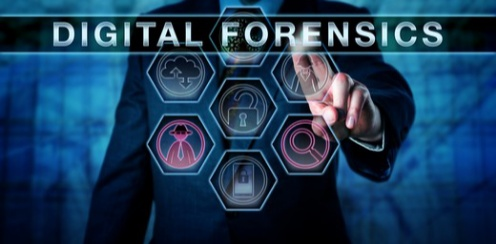
\includegraphics[width=0.5\textwidth]{For.jpeg}
			% Ligne séparatrice
			\noindent\rule{0.9\textwidth}{0.8pt}\\
			\vspace{1.5cm}
			
			% Informations étudiant
			\begin{tabular}{@{}>{\bfseries}l l@{}}
				\vspace{0.5cm}
				Réalisé par : & \textbf{NANTIA ZAGUE AXEL FRISKYL} \\
				\vspace{0.5cm}
				Matricule : & \textbf{22P105} \\
				\vspace{0.5cm}
				Spécialité : & \textbf{Cybersécurité et Investigation Numérique (CIN)} \\
				\vspace{0.5cm}
				UE : & \textbf{Introduction aux techniques de l'Investigations Numériques} \\
				\vspace{0.5cm}
				Sous la supervision de : & \textbf{Mr. MINKA MI NGUIDJOI Thierry Emmanuel} \\
				\vspace{0.5cm}
				Année académique : & \textbf{2025/2026} \\
			\end{tabular}
			
		\end{titlepage}
		
		% Page de garde sans en-tête
		\thispagestyle{empty}
		\newpage
	
	\begin{titlepage}
		\centering
		\vspace*{1cm}
		{\LARGE\bfseries Rapport de Laboratoire :\\Configuration Réseau et Simulation de Ransomware\par}
		\vspace{1.5cm}
		{\large Cours : Sécurité des Réseaux et Systèmes\par}
		\vspace{1cm}
		{\large Date : \today\par}
		\vspace{2cm}
		\begin{abstract}
			Ce rapport présente les travaux réalisés dans le cadre de deux laboratoires de sécurité informatique. Le premier labo concerne la configuration d'un environnement réseau sécurisé avec GNS3, intégrant un firewall FortiGate et une DMZ. Le deuxième labo porte sur le développement et le test d'un ransomware simulé pour comprendre les mécanismes de cette menace cybernétique.
		\end{abstract}
		\vfill
	\end{titlepage}
	
	\tableofcontents
	\newpage
	
	\section{Lab 1 – Configuration d'un environnement réseau fonctionnel et sécurisé}
	
	\subsection{Objectif du laboratoire}
	Ce laboratoire consistait à concevoir un réseau sous GNS3 incluant plusieurs machines virtuelles (Windows, Linux, Kali), un routeur, un firewall FortiGate, et la segmentation en sous-réseaux. L'objectif était de maîtriser la création d'une DMZ, le paramétrage du routage et la sécurisation par firewall, tout en maintenant la connectivité sur les services autorisés entre les différentes zones.
	
	\subsection{Architecture du réseau}
	
	\begin{figure}[H]
		\centering
		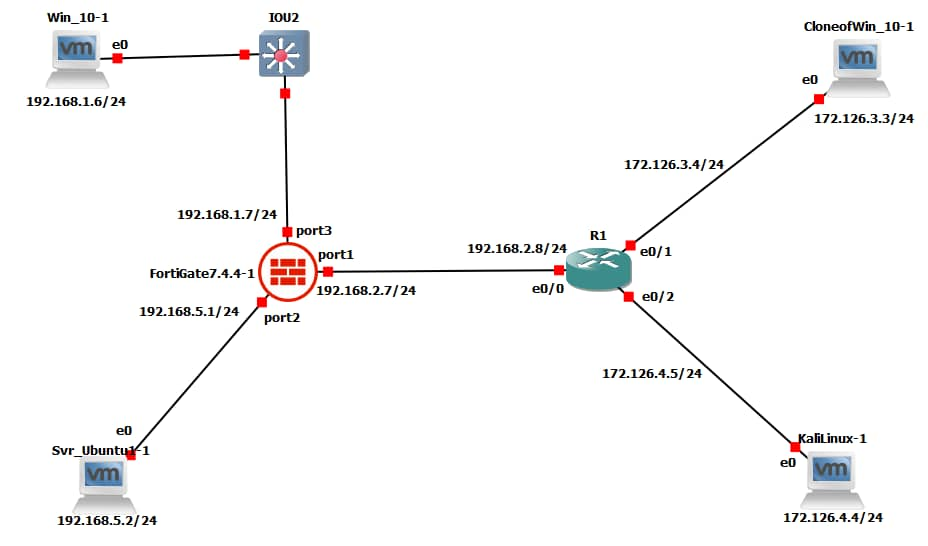
\includegraphics[width=0.9\textwidth]{image0.jpeg}
		\caption{Schéma de l'architecture réseau réalisée sous GNS3}
		\label{fig:architecture}
	\end{figure}
	
	L'architecture réalisée est fidèle à celle proposée dans l'énoncé. Elle inclut les composants suivants :
	
	\begin{itemize}
		\item \textbf{VM Windows 10} : 192.168.1.6/24 (réseau local)
		\item \textbf{Serveur Ubuntu} : 192.168.5.2/24 (DMZ)
		\item \textbf{Firewall FortiGate} : 
		\begin{itemize}
			\item Port1 : 192.168.2.7/24
			\item Port2 : 192.168.5.1/24
			\item Port3 : 192.168.1.7/24
		\end{itemize}
		\item \textbf{Routeur R1} : Interfaces e0/0, e0/1, e0/2 pour interconnecter les zones internes et externes
		\item \textbf{Kali Linux} : 172.126.4.4/24 (machine d'attaque)
		\item \textbf{CloneWindows} : 172.126.3.3/24 (cible additionnelle)
	\end{itemize}
	
	Le schéma, bien segmenté, permet de contrôler les accès entre la DMZ, le réseau local (LAN), et les zones « extérieures », comme demandé par le lab.
	
	\subsection{Configurations et vérifications réalisées}
	
	\subsubsection{Politique sur le firewall}
	Sur le FortiGate, chaque port a été configuré avec les règles adaptées :
	\begin{itemize}
		\item La DMZ n'est accessible que via certains services (HTTP/HTTPS)
		\item La VM Windows bloque tout trafic non nécessaire
		\item Les règles inter-zones segmentent correctement les réseaux internes, DMZ et zones d'attaque
	\end{itemize}
	
	\subsubsection{Routage}
	Le routeur R1 a été configuré pour faire du routage entre les différents sous-réseaux. Les routes statiques ont été définies pour permettre la communication entre le LAN, la DMZ, et la zone d'attaque, tout en respectant l'isolation.
	
	\subsubsection{Adressage IP}
	Toutes les interfaces ont reçu des adresses IP cohérentes avec le plan d'adressage fourni. Les VLAN et sous-réseaux sont correctement séparés.
	
	\subsubsection{Tests de connectivité}
	Des tests ping et d'accès HTTP/HTTPS ont été menés pour valider la configuration et l'application correcte des règles de sécurité.
	
	\subsection{Conclusion du Lab 1}
	L'architecture réseau a été correctement implémentée avec une segmentation efficace des différentes zones de sécurité. Les règles firewall appliquées permettent un contrôle granulaire des accès tout en maintenant la fonctionnalité des services essentiels.
	
	\section{Lab 2 – Création et test d'un ransomware simulé}
	
	\subsection{Objectif du laboratoire}
	Ce laboratoire demandait de développer sous Kali Linux un script de ransomware simulant le chiffrement (en renommant les fichiers avec une extension, par exemple ".locked"), puis de transformer ce script en exécutable Windows (.exe avec PyInstaller), et enfin de tester son propagation sur une VM Windows soit par email, soit par téléchargement malveillant hébergé sur Kali.
	
	\begin{figure}[H]
		\centering
		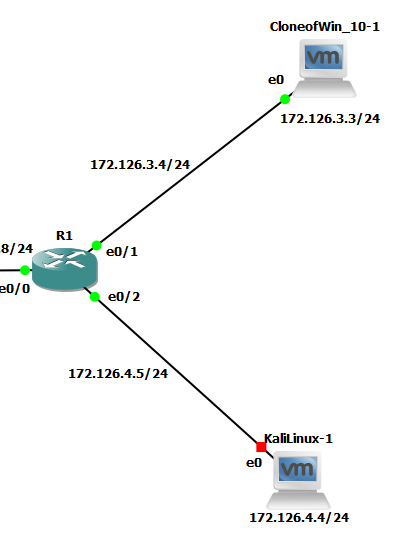
\includegraphics[width=0.7\textwidth]{cap.PNG}
		\caption{Test du ransomware sur la VM CloneWindows}
		\label{fig:ransomware}
	\end{figure}
	
	\subsection{Développement du ransomware}
	
	\subsubsection{Implémentation technique}
	Le ransomware a été développé en Python sur Kali Linux avec les caractéristiques suivantes :
	\begin{itemize}
		\item Accès à la machine cible via les informations d'authentification (nom, utilisateur, mot de passe)
		\item Chiffrement simulé par renommage des fichiers avec une extension ".locked"
		\item Génération d'un message de rançon avec instructions de paiement
		\item Transformation en exécutable Windows via PyInstaller
	\end{itemize}
	
	\subsubsection{Résultats des tests}
	Le ransomware a été testé avec succès sur la VM CloneWindows :
	\begin{itemize}
		\item Le script a correctement fonctionné et a "chiffré" les fichiers cibles
		\item Le message de rançon a été affiché avec les informations bancaires demandées
		\item La simulation a permis de comprendre les mécanismes d'infection
	\end{itemize}
	
	\subsection{Limitations rencontrées}
	\begin{itemize}
		\item \textbf{Connectivité internet} : Impossible de réaliser la propagation par email en raison de l'absence de connectivité internet des machines virtuelles
		\item \textbf{Bibliothèques manquantes} : Difficultés à télécharger les dépendances nécessaires pour certaines fonctionnalités avancées
		\item \textbf{Fonctionnalités réduites} : Le ransomware développé reste basique comparé aux véritables menaces
	\end{itemize}
	
	\subsection{Conclusion du Lab 2}
	Ce laboratoire a permis de comprendre les principes fondamentaux du fonctionnement des ransomwares et les défis techniques liés à leur développement. La simulation a mis en évidence l'importance des mesures de protection et de détection contre ce type de menace.
	
	\section{Conclusion générale}
	
	Les deux laboratoires ont permis d'acquérir des compétences pratiques en sécurité réseau et en analyse de menaces cybernétiques. Le premier labo a renforcé la compréhension des architectures réseau sécurisées et des politiques firewall, tandis que le deuxième a offert une perspective concrète sur le fonctionnement des ransomwares.
	
	Ces expériences pratiques sont essentielles pour développer une approche proactive de la sécurité informatique, combinant à la fois la prévention technique et la compréhension des tactiques adverses.
	
\end{document}